\documentclass[../main.tex]{subfiles}

\begin{document}
	\section{Retroazione algebrica sull'uscita}
		Consideriamo il sistema $ S $ dove dall'uscita eliminiamo il termine $ Du $ per evitare i possibili loop algebrici che si avrebbero con una retroazione:
		\[
			S:
			\begin{cases}
				\dot x = Ax+Bu\\
				y = Cx
			\end{cases}
		\]
	
		Effettuiamo la retroazione $ u = Ky +v $:
		\[
			S^{*}:
			\begin{cases}
				\dot x = Ax + B(Ky+v) = (A+BKC)x + Bv = A^{*}x + Bv\\
				y = Cx
			\end{cases}
		\]
		
		\begin{figure}[H]
			\centering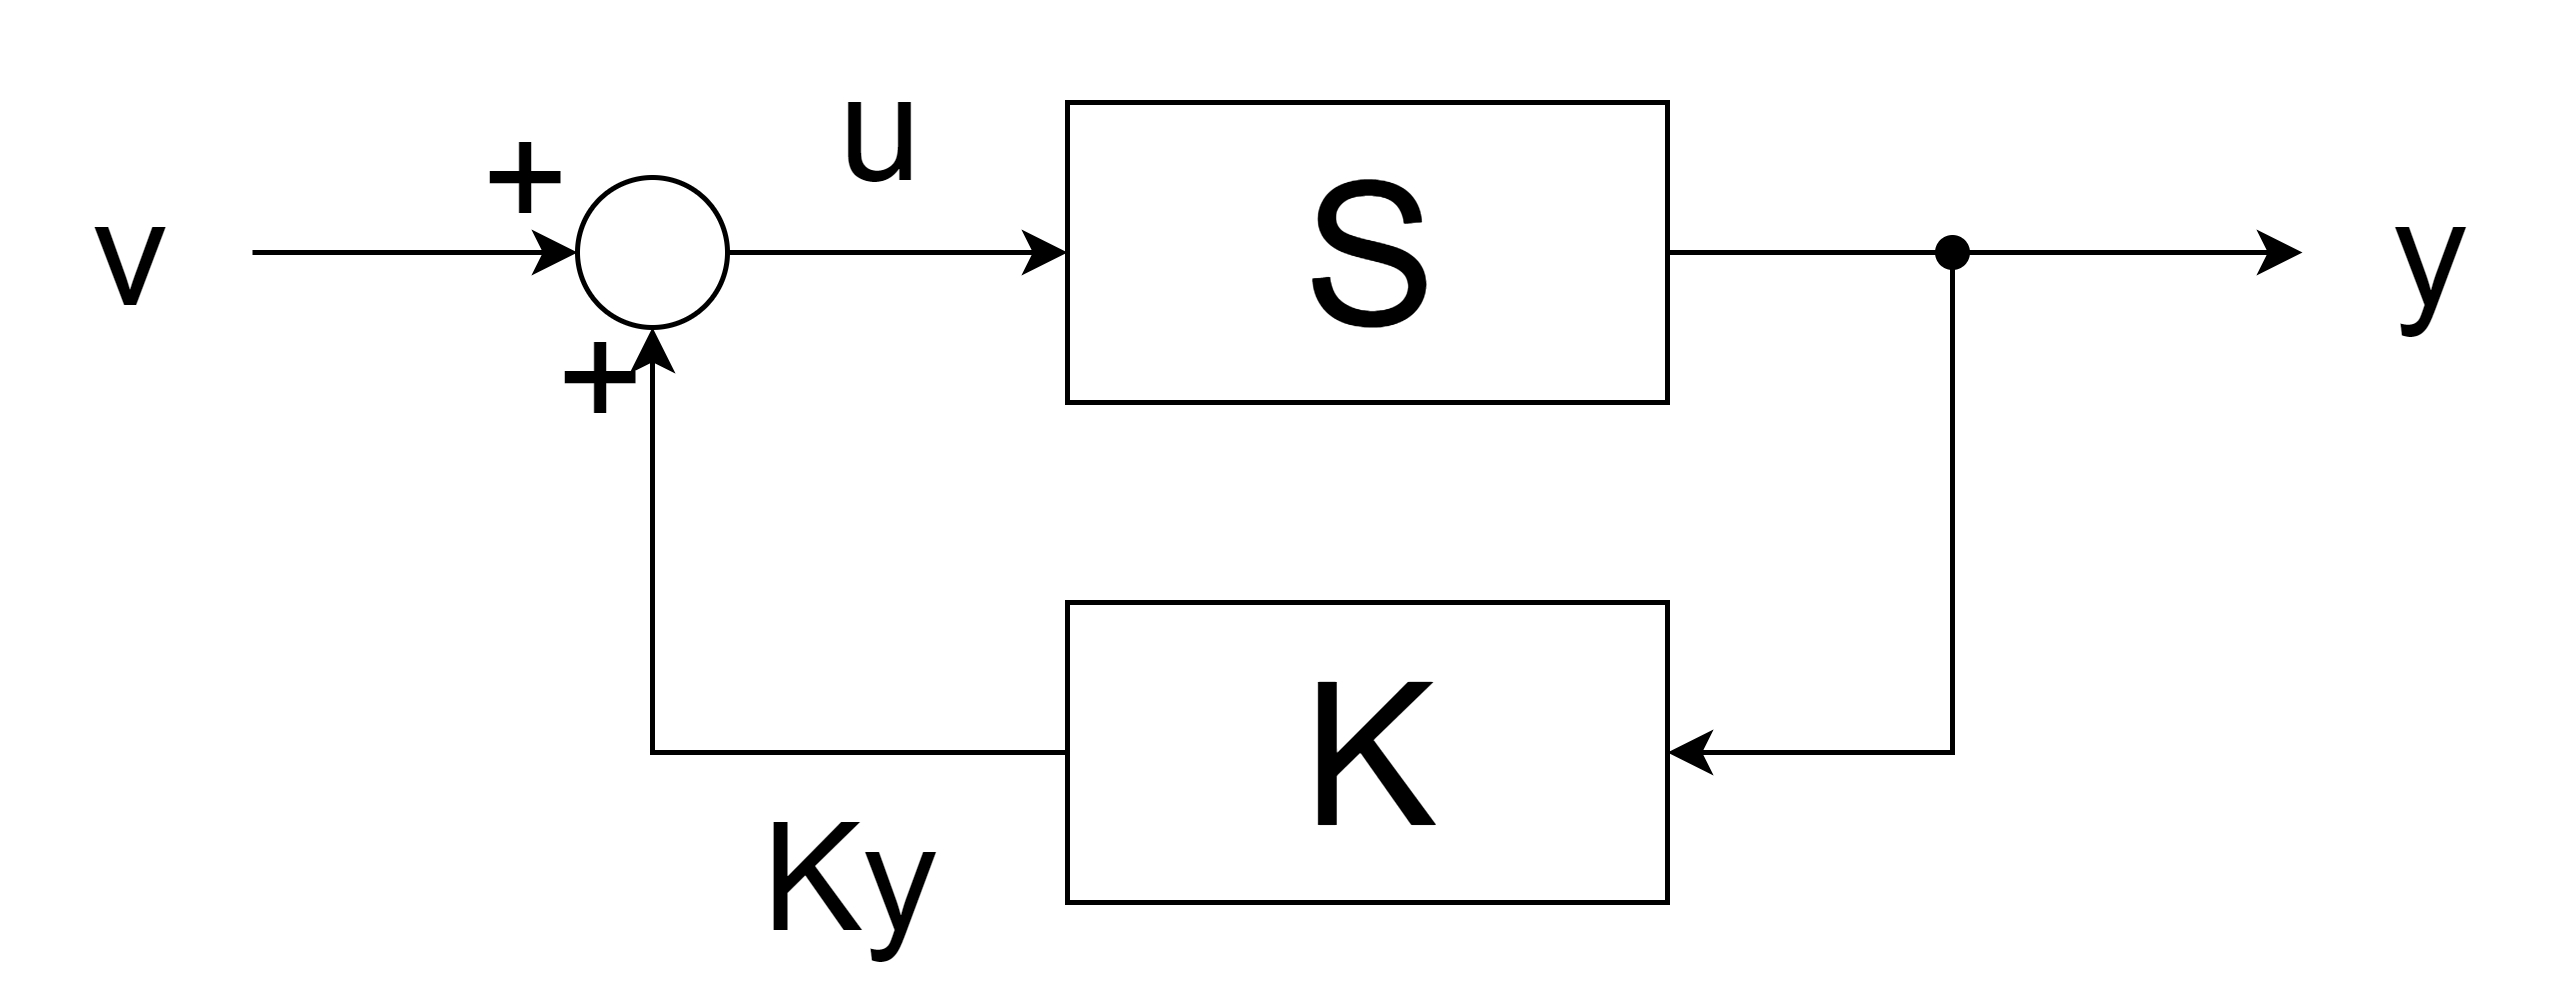
\includegraphics[width=.5\textwidth]{retroazione_algebrica_uscita/retroazione_algebrica_uscita}
		\end{figure}
	
		Si pu\'o osservare che:
		\begin{itemize}
			\item 
				la retroazione appena effettuata \'e simile alla retroazione algebrica sullo stato $ u = \hat K x+ v $: infatti la retroazione algebrica sull'uscita \'e una particolare retroazione algebrica sullo stato, ma con pi\'u vincoli.
			\item 
				la retroazione algebrica sullo stato non modifica le propriet\'a di raggiungibilit\'a.
		\end{itemize}
		Grazie a queste due propriet\'a otteniamo che:
		\begin{center}
			\fbox{
				\begin{minipage}{.8\linewidth}
					La retroazione algebrica sull'uscita NON modifica le propriet\'a di controllabilit\'a del sistema
				\end{minipage}
			}
		\end{center}
		Analogamente per l'osservabilit\'a:
		\begin{center}
			\fbox{
				\begin{minipage}{.8\linewidth}
					La retroazione algebrica sull'uscita NON modifica le propriet\'a di osservabilit\'a del sistema
				\end{minipage}
			}
		\end{center}
		\textbf{Dimostriamo} quest'ultima propriet\'a:
		supponiamo che $ \hat{\vec x} \in X_{NO}^{*} $ cio\'e che $ \hat{\vec x} $ sia indistinguibile dallo stato zero dopo la retroazione, dove
		\[
			X_{NO}^{*} = ker(Q^{*}) = ker
			\begin{bmatrix}
				C\\
				CA^{*}\\
				C(A^{*})^2\\
				\vdots\\
				C(A^{*})^{n_x-1}
			\end{bmatrix} =
			\begin{bmatrix}
				C\\
				C(A+BKC)\\
				C(A+BKC)^2\\
				\vdots\\
				C(A+BKC)^{n_x-1}
			\end{bmatrix}
		\]
		quindi per definizione di kernel $ Q^{*} \vec x = 0 $:
		\[
			\begin{bmatrix}
				C\\
				C(A+BKC)\\
				C(A+BKC)^2\\
				\vdots\\
				C(A+BKC)^{n_x-1}
			\end{bmatrix} \hat{\vec x} =
			\begin{bmatrix}
				0\\
				0\\
				0\\
				\vdots\\
				0
			\end{bmatrix}
		\]
		effettuiamo il conto riga per riga:
		\begin{enumerate}
			\item
				$ C \hat{\vec x} = 0 $
			\item
				$ C(A+BKC) \hat{\vec x} = CA \hat{\vec x} + CBK\underbrace{C \hat{\vec x}}_{=0} = 0 \quad\Rightarrow\quad CA \hat{\vec x} = 0 $
			\item 
				$ C(A+BKC)^2 \hat{\vec x} = C(A^2 + ABKC + BKCA + BKCBKC) \hat{\vec x} = $
				\\
				$ = CA^2 \hat{\vec x} + ABK \underbrace{C \hat{\vec x}}_{=0} + BK\underbrace{CA \hat{\vec x}}_{=0} + BKCBK\underbrace{C \hat{\vec x}}_{=0} = CA^2 \hat{\vec x} $
			\item $ \dots $
			\item[n.]
				$ C A^{n_x-1} \hat{\vec x} = 0 $
		\end{enumerate}
		\[
			\Rightarrow\quad
			\begin{bmatrix}
				C\\
				CA\\
				\vdots\\
				CA^{n_x-1}
			\end{bmatrix} 
			= Q \hat{\vec x} = \hat{\vec x} = 0
			\quad\Rightarrow\quad
			\hat{\vec x} \in Ker(Q) = X_{NO}
		\]
		c.v.d.
		
	\subsection{Polinomio caratteristico}
		Supponiamo di effettuare la decomposizione di Kalmann al sistema retroazionato:
		\[
			\tilde S^{*}:
			\begin{cases}
				\dot z = (\tilde A + \tilde B K \tilde C)z + \tilde B v = \tilde A^{*} z + \tilde v
				\\
				y = \tilde C z
			\end{cases}
		\]
		\[
			\tilde B K \tilde C =
			\begin{bmatrix}
				\tilde B_1\\
				\tilde B_2\\
				0\\
				0
			\end{bmatrix} K
			\begin{bmatrix}
				0\\
				\tilde C_2\\
				0\\
				\tilde C_4
			\end{bmatrix} =
			\begin{bmatrix}
				0 & \tilde B_1 K \tilde C_2 & 0 & \tilde B_1 K \tilde C_4\\
				0 & \tilde B_2 K \tilde C_2 & 0 & \tilde B_2 K \tilde C_4\\
				0 & 0 & 0 & 0\\
				0 & 0 & 0 & 0
			\end{bmatrix}
		\]
		\[
			\tilde A^{*} =
			\begin{bmatrix}
				\tilde A_{11} & (\tilde A_{12} + \tilde B_1 K \tilde C_2) & \tilde A_{13} & (\tilde A_{14} + \tilde B_1 K \tilde C_4)\\
				0 & (\tilde A_{22} + \tilde B_2 K \tilde C_2) & 0 & (\tilde A_{24} + \tilde B_2 K \tilde C_4)\\
				0 & 0 & \tilde A_{33} & \tilde A_{34}\\
				0 & 0 & 0 & \tilde A_{44}
			\end{bmatrix}
		\]
		
		$ \varphi^{*}(s) $ \'e il polinomio caratteristico associato $ A + BKC $. $ \tilde \varphi^{*}(s) $ \'e il polinomio caratteristico del sistema retroazionato decomposto con Kalmann, associato a $ \tilde A + \tilde B K \tilde C $. Nonostante ci\'o il polinomio caratteristico \'e invariante ai cambiamenti di base:
		\[
			\varphi^{*}(s) = \tilde \varphi^{*}(s)
		\]
		
		Inoltre la matrice $ \tilde A^{*} $ ha mantenuto la struttura triangolare a blocchi:
		\[
			\varphi^{*}(s) = \tilde \varphi^{*}(s) = det(sI-\tilde A_{11}) \cdot det[sI-(\tilde A_{22} + \tilde B_2 K \tilde C_2)] \cdot det(sI-\tilde A_{33}) \cdot det(sI-\tilde A_{44})
		\]
		Rispetto a quanto avevamo trovato nella \hyperref[sec:decomp_kalmann_polinomio]{decomposizione di Kalmann}, solo il secondo fattore \'e stato modificato dalla retroazione:
		\begin{center}
			\fbox{
				\begin{minipage}{.8\linewidth}
					La retroazione algebrica sull'uscita pu\'o modificare (non sempre a piacere) solo la parte controllabile e osservabile del sistema.
				\end{minipage}
			}
		\end{center}
		Vengono "modificati" e non "assegnati a piacere" gli autovalori controllabili \textbf{e} osservabili a causa del vincolo imposto dalla matrice $ C $. Se $ rank(C) = n_x $ allora la retroazione sull'uscita equivale alla retroazione algebrica sullo stato.
		
		\begin{mdframed}[style=Exercise]
			\begin{Exercise}[title={Retroazione algebrica sull'uscita}, difficulty=1]
				\[
					\begin{cases}
						\dot x=
						\begin{bmatrix}
							0 & 1\\
							0 & 0
						\end{bmatrix} x+
						\begin{bmatrix}
							0\\
							1
						\end{bmatrix} u
						\\[.5cm]
						y =
						\begin{bmatrix}
							1 & 0
						\end{bmatrix} x
					\end{cases}
				\]
				Il sistema ha $ n_x = 2 $, ma la retroazione sull'uscita \'e $ u = Ky + v $ con $ K \in \R $ (scalare): \'e evidente che con la sola variabile $ K $ non posso fissare entrambi gli autovalori del sistema.
				
				Studiamo velocemente il sistema:
				\begin{itemize}
					\item 
						\[
							(sI-A)^{-1} =
							\begin{bmatrix}
								s & -1\\
								0 & s
							\end{bmatrix}^{-1} =
							\begin{bmatrix}
								\dfrac{1}{s} & \dfrac{1}{s^2}\\[.5cm]
								0 & \dfrac{1}{s}
							\end{bmatrix}
							\quad\Rightarrow\quad
							\varphi(s) = mcm\left\lbrace s, s, s^2 \right\rbrace = s^2
						\]
					\item 
						poich\'e $ m(s) \subseteq\cdot \varphi(s) $, i possibili polinomi minimi sono: $ s $ e $ s^2 $. Verifichiamo se $ s $ \'e polinomio annullante per $ A $, cio\'e $ m(A) = 0 $. Tuttavia $ A \neq 0 $, $ A $ non \'e una matrice nulla, quindi significa che $ m(s) = s^2 $ (infatti $ A^2 = 0 $).
					\item 
						l'unica radice di $ m(s) $ \'e a $ \Re = 0 $ con molteplicit\'a $ 2 $ quindi il sistema \'e instabile.
					\item 
						controllabilit\'a:
						\[
							(sI-A)^{-1}B=
							\begin{bmatrix}
								\dfrac{1}{s} & \dfrac{1}{s^2}\\[.5cm]
								0 & \dfrac{1}{s}
							\end{bmatrix}
							\begin{bmatrix}
								0\\
								1
							\end{bmatrix} =
							\begin{bmatrix}
								\dfrac{1}{s^2}\\[.5cm]
								\dfrac{1}{s}
							\end{bmatrix}
						\]
						Trucchetto: se nella matrice compare un denominatore di grado massimo, allora esso sar\'a il polinomio caratteristico: $ \varphi_C(s) = s^2 $. Inoltre $ \varphi_C(s) \equiv m_C(s) $.\\
						Oppure col teorema di Kalmann:
						\[
							P =
							\begin{bmatrix}
								0 & 1\\
								1 & 0
							\end{bmatrix}
						\]
						Il sistema \'e completamente controllabile.
					\item 
						osservabilit\'a:
						\[
							C(sI-A)^{-1} = 
							\begin{bmatrix}
								\dfrac{1}{s} & \dfrac{1}{s^2}
							\end{bmatrix}
							\quad\Rightarrow\quad \varphi_O(s) = s^2
						\]
						oppure
						\[
							Q =
							\begin{bmatrix}
								1 & 0\\
								0 & 1
							\end{bmatrix}
						\]
						il sistema \'e completamente osservabile.
				\end{itemize}
				\begin{enumerate}
					\item 
						\'E possibile rendere il sistema asintoticamente stabile con una retroazione algebrica sull'uscita?\\
						Per vedere ci\'o calcoliamo il polinomio caratteristico del sistema retroazionato:
						\[
							A^{*}=(A+BKC)
							\begin{bmatrix}
								0 & 1\\
								0 & 0
							\end{bmatrix} +
							\begin{bmatrix}
								0\\
								1
							\end{bmatrix} K
							\begin{bmatrix}
								1 & 0
							\end{bmatrix} =
							\begin{bmatrix}
								0 & 1\\
								0 & 0
							\end{bmatrix} +
							\begin{bmatrix}
								0 & 0\\
								K & 0
							\end{bmatrix} =
							\begin{bmatrix}
								0 & 1\\
								K & 0
							\end{bmatrix}
						\]
						\[
							\varphi^{*}(s) = det(sI-A^{*}) = det
							\begin{bmatrix}
								s & -1\\
								-K & s
							\end{bmatrix} = s^2 - K
						\]
						per $ K \geq 0 $ il sistema resta instabile, mentre per $ K < 0 $ \'e semplicemente stabile.
					\item 
						Con la retroazione \'e possibile assegnare a piacere qualche autovalore?
						S\'i purch\'e i coefficienti del polinomio che vogliamo ottenere siano reali.
				\end{enumerate}
			\end{Exercise}
		\end{mdframed}
	
	\subsection{Stabilit\'a BIBO}
		\[
			\text{stabilit\'a BIBO}\quad\Rightarrow\quad \varphi_{CO}(s)\ \text{non ha radici a}\ \Re \geq 0
		\]
		
		$ \varphi_{CO}(s) $ \'e il polinomio caratteristico associato a $ T(s) $ prima della retroazione. Se si pu\'o calcolare $ T^{*}(s) = T_{yv}(s) $ (dopo la retroazione), allora $ \varphi^{*}_{CO}(s) $ sar\'a il polinomio caratteristico associato a $ T^{*}(s) $.
		
		\begin{mdframed}[style=Exercise]
			\begin{Exercise}[title={Studio retr. alg. sull'uscita con l'algebra dei blocchi}]
				Riprendiamo l'esercizio precedente e calcoliamo la funzione di trasferimento:
				\[
					C(sI-A)^{-1}B +D =
					\begin{bmatrix}
						1 & 0
					\end{bmatrix}
					\begin{bmatrix}
						\dfrac{1}{s} & \dfrac{1}{s^2}
						\\[1em]
						0 & \dfrac{1}{s}
					\end{bmatrix}
					\begin{bmatrix}
						0\\
						1
					\end{bmatrix} =
					\begin{bmatrix}
						1 & 0
					\end{bmatrix}
					\begin{bmatrix}
						\dfrac{1}{s^2}
						\\[1em]
						\dfrac{1}{s}
					\end{bmatrix} =
					\dfrac{1}{s^2}
				\]
				Applichiamo la retroazione algebrica sull'uscita:
				\[
					T_{yv}(s) = \dfrac{\dfrac{1}{s^2}}{1-K\dfrac{1}{s^2}} = \dfrac{\dfrac{1}{s^2}}{\dfrac{s^2-K}{s^2}} = \dfrac{1}{s^2 - K}
				\]
				\[
					\Rightarrow\quad \varphi^{*}_{CO}(s) = s^2 -K
				\]
				Abbiamo ottenuto molto pi\'u facilmente lo stesso risultato di prima.
			\end{Exercise}
		\end{mdframed}

		\begin{mdframed}[style=Exercise]
			\begin{Exercise}[title={Studio stabilit\'a BIBO dopo retroazione sull'uscita}, difficulty=1]
				\[
					T(s) = \dfrac{1}{s(s-1)}
				\]
				si tratta di un sistema non stabile BIBO perch\'e i poli di $ T(s) $ sono $ 0 $ e $ 1 $ (una radice ha $ \Re > 0 $). Con la retroazione sull'uscita si pu\'o rendere il sistema stabile BIBO?
				\[
					T^{*}(s) = \dfrac{\dfrac{1}{s(s-1)}}{1-\dfrac{K}{s(s-1)}} = \dfrac{1}{s^2-s-K}
				\]
				$ \exists K $ tale che i poli di $ T^{*}(s) $ siano tutti a $ \Re < 0 $?\\
				Con la regola di Cartesio si trova subito una variazione (tra $ s^2 $ e $ -s $) che determina la presenza di almeno una radice a $ \Re > 0 $. Quindi il sistema retroazionato non \'e stabile BIBO per nessun $ K $. Analizziamo comunque i casi al variare di $ K $:
				\begin{itemize}
					\item $ K < 0 $: due variazioni $ \quad\Rightarrow\quad $ due radici a $ \Re > 0 $
					\item $ K > 0 $: una variazione $ \quad\Rightarrow\quad $ una radice a $ \Re > 0 $ e una radice a $ \Re < 0 $
					\item $ K = 0 $: una radice a $ \Re > 0 $ e una radice a $ \Re = 0 $
				\end{itemize}
			\end{Exercise}
		\end{mdframed}
\end{document}